\documentclass[10pt,aspectratio=169]{beamer}

\usetheme{metropolis}
\usepackage{appendixnumberbeamer}

\usepackage{booktabs}
\usepackage{tabularx}
\usepackage{multirow}
\usepackage{colortbl}
\usepackage{graphicx}
\usepackage{tikz}
\usepackage{pgfplots}
\pgfplotsset{compat=1.16}
\usetikzlibrary{shapes,arrows,positioning,calc}

\usepackage{amsmath}
\usepackage{amssymb}
\usepackage{pifont}

% Colors
\definecolor{winnergreen}{RGB}{39, 174, 96}
\definecolor{warningorange}{RGB}{230, 126, 34}
\definecolor{errorred}{RGB}{192, 57, 43}
\definecolor{niceblue}{RGB}{52, 152, 219}
\definecolor{lightgray}{RGB}{245, 245, 245}

\title{RRMC — Week 5}
\subtitle{AllSuspects, Ensemble, and DQS on DC \& GN}
\date{2026-02-06}
\author{}
\institute{Qwen 2.5 7B Instruct via OpenRouter}

\begin{document}

\maketitle

%==============================================================================
\section{Detective Cases — Stopping Rules}
%==============================================================================

\begin{frame}{DC: All Methods Head-to-Head (20 puzzles)}
  \begin{table}
    \centering
    \small
    \begin{tabular}{lcccl}
      \toprule
      \textbf{Method} & \textbf{Accuracy} & \textbf{Avg Turns} & \textbf{Cost} & \textbf{Note} \\
      \midrule
      \rowcolor{winnergreen!15}
      CIP-Lite        & \textbf{45\%} & 1.4  & 1$\times$   & \textit{best overall} \\
      KnowNo          & 40\%          & 1.0  & 1$\times$   & stops T1 always \\
      Self-Consistency & 35\%         & 1.4  & 1$\times$   & \\
      Semantic Entropy & 35\%         & 1.4  & 1$\times$   & \\
      Fixed Turns (10) & 30\%         & 10.0 & 1$\times$   & \\
      Verb.\ Confidence & 30\%        & 23.1 & 1$\times$   & never stops \\
      MI-Only          & 25\%         & 4.1  & 1$\times$   & MI=0 at T1 \\
      \midrule
      AllSuspects+CIP  & 15\%         & 6.6  & 1$\times$   & \textcolor{errorred}{$\downarrow$30pp} \\
      Ensemble+AS+CIP  & 25\%         & 7.0  & 8$\times$   & \textcolor{errorred}{$\downarrow$20pp} \\
      \midrule
      \rowcolor{winnergreen!20}
      \textbf{DQS + Fixed(10)} & \textbf{60\%} & \textbf{10.0} & \textbf{11$\times$} & \textcolor{winnergreen}{\textbf{$\uparrow$30pp}} \\
      \bottomrule
    \end{tabular}
  \end{table}

  \vspace{0.2cm}

  \begin{exampleblock}{}
    DQS is the \textbf{only method that improves} over baseline: 30\% $\rightarrow$ 60\%.
    AllSuspects/Ensemble both degrade.
  \end{exampleblock}
\end{frame}

%==============================================================================
\section{The Turn-1 Paradox}
%==============================================================================

\begin{frame}{CIP-Lite Stops at Turn 1 — And That's the Best Strategy}

  \begin{columns}[T]
    \begin{column}{0.45\textwidth}
      \begin{table}
        \centering
        \small
        \begin{tabular}{lcc}
          \toprule
          \textbf{Subgroup} & \textbf{n} & \textbf{Acc} \\
          \midrule
          \rowcolor{winnergreen!15}
          CIP-Lite stops T1 & 15 & \textbf{47\%} \\
          CIP-Lite stops T2+ & 5 & 40\% \\
          \midrule
          AllSuspects (T5+) & 20 & \textcolor{errorred}{15\%} \\
          \bottomrule
        \end{tabular}
      \end{table}

      \vspace{0.3cm}

      \textbf{AllSuspects degradation ratio:}

      \begin{itemize}
        \item 7 correct $\rightarrow$ wrong
        \item 1 wrong $\rightarrow$ correct
        \item \textbf{Net: $-$6 puzzles}
      \end{itemize}
    \end{column}

    \begin{column}{0.52\textwidth}
      \begin{block}{Why T1 works}
        CIP-Lite samples $k{=}8$ answers from the case background alone.
        When all 8 agree (set size = 1), the model \textbf{consistently}
        identifies the same suspect from the description.

        \vspace{0.2cm}

        This is genuine comprehension of the case text —
        the model's \textbf{strongest signal}.
      \end{block}

      \vspace{0.2cm}

      \begin{alertblock}{Why more turns hurt}
        NPC responses are LLM-generated, generic alibis
        (``I was at home''). Every extra turn adds \textbf{noise}
        that overwrites the correct first impression.
      \end{alertblock}
    \end{column}
  \end{columns}
\end{frame}

%==============================================================================
\section{Why AllSuspects \& Ensemble Fail}
%==============================================================================

\begin{frame}{AllSuspects Failure: Puzzle 1 — Correct $\rightarrow$ Wrong}

  \small
  Victim: Dr.\ Jonathan Reed \quad | \quad Guilty: \textbf{Evelyn Carter (\#0)}

  \vspace{0.2cm}

  \begin{columns}[T]
    \begin{column}{0.48\textwidth}
      \textbf{Baseline}: \textcolor{winnergreen}{\checkmark} Evelyn Carter (T1)

      \vspace{0.1cm}

      Reads case background $\rightarrow$ immediately identifies Carter.

      \vspace{0.3cm}

      \textbf{AllSuspects}: \textcolor{errorred}{\ding{55}} Samantha Greene (T6)

      \vspace{0.1cm}

      Forced to question all 5 suspects:

      \vspace{0.1cm}
      \footnotesize
      \begin{tabular}{rl}
        T1: & Carter --- ``I was at home, reviewing data.'' \\
        T2: & Whitmore --- ``I was at home, relaxing.'' \\
        T3: & Collins --- ``I was at home, making sense.'' \\
        T4: & Donovan --- ``I was at home, relaxing.'' \\
        T5: & Greene --- ``I was at home watching a movie, \\
            & \quad but I heard a \textbf{sighting near the park}.'' \\
      \end{tabular}
    \end{column}

    \begin{column}{0.48\textwidth}
      \begin{alertblock}{What went wrong}
        Every suspect says ``I was at home.''

        \vspace{0.1cm}

        Greene adds one irrelevant detail (``sighting near the park'')
        $\rightarrow$ model latches onto it as evidence
        $\rightarrow$ \textbf{changes answer from Carter to Greene}.

        \vspace{0.1cm}

        The NPC responses carry \textbf{no signal} — all generic alibis.
        The model over-interprets minor phrasing differences.
      \end{alertblock}

      \vspace{0.2cm}

      \begin{block}{Pattern}
        7 of 20 puzzles: baseline correct, AllSuspects flipped it wrong.
        Only 1 puzzle went the other direction.
        \textbf{Ratio: 7:1 against.}
      \end{block}
    \end{column}
  \end{columns}
\end{frame}

\begin{frame}{Ensemble Failure: Puzzle 6 — 80\% Confident and Wrong}

  \small
  Guilty: \textbf{Michael Turner (\#1)}

  \vspace{0.2cm}

  \begin{columns}[T]
    \begin{column}{0.48\textwidth}
      \begin{table}
        \centering
        \small
        \begin{tabular}{lccc}
          \toprule
          \textbf{Method} & \textbf{Pred} & \textbf{Correct?} \\
          \midrule
          Baseline & \#1 Turner & \textcolor{winnergreen}{\checkmark} \\
          AllSuspects & \#1 Turner & \textcolor{winnergreen}{\checkmark} \\
          \rowcolor{errorred!15}
          Ensemble & \#0 Carter & \textcolor{errorred}{\ding{55}} \\
          \bottomrule
        \end{tabular}
      \end{table}

      \vspace{0.2cm}

      Ensemble consensus: \textbf{4/5 trajectories} (80\%) voted for
      the \textbf{wrong} suspect.

      \vspace{0.2cm}

      Both baseline and AllSuspects got it right independently —
      the ensemble \textbf{killed} the correct answer.
    \end{column}

    \begin{column}{0.48\textwidth}
      \begin{alertblock}{What happened}
        All 6 trajectories run at the \textbf{same temperature}\footnotemark.
        The model has a systematic bias toward Carter
        (most narrative connection to victim).

        \vspace{0.1cm}

        4 of 5 valid trajectories follow the same
        reasoning path $\rightarrow$ same wrong answer.

        \vspace{0.1cm}

        Majority vote \textbf{amplifies} the bias
        instead of correcting it.
      \end{alertblock}

      \vspace{0.2cm}

      \begin{block}{Broader pattern}
        Ensemble consensus anti-correlates with correctness.
        4/6 consensus: only 17\% accurate.
        No puzzle reached 5/6 or 6/6.
      \end{block}
    \end{column}
  \end{columns}

  \footnotetext{Temperature diversity was configured but not applied due to a wiring bug. All trajectories ran at temp=0.7.}
\end{frame}

%==============================================================================
\section{DQS — Deliberative Question Selection}
%==============================================================================

\begin{frame}{DQS: Can Better Questions Help?}

  Instead of improving \textit{when} to stop, improve \textit{what} to ask.

  \vspace{0.3cm}

  \begin{center}
  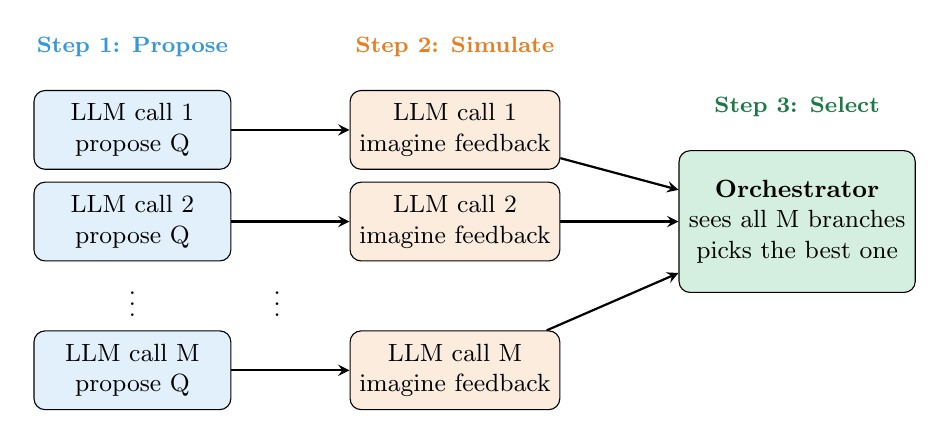
\begin{tikzpicture}[
    node distance=0.6cm and 1.2cm,
    block/.style={rectangle, draw, rounded corners, minimum height=1cm,
                  minimum width=2.5cm, align=center, font=\small},
    arr/.style={->, thick, >=stealth},
  ]
    % Step 1
    \node[block, fill=niceblue!15] (p1) {LLM call 1\\propose Q};
    \node[block, fill=niceblue!15, below=0.15cm of p1] (p2) {LLM call 2\\propose Q};
    \node[below=0.05cm of p2, font=\small] (dots1) {$\vdots$};
    \node[block, fill=niceblue!15, below=0.05cm of dots1] (pm) {LLM call M\\propose Q};

    % Step 2
    \node[block, fill=warningorange!15, right=1.5cm of p1] (s1) {LLM call 1\\imagine feedback};
    \node[block, fill=warningorange!15, right=1.5cm of p2] (s2) {LLM call 2\\imagine feedback};
    \node[right=1.5cm of dots1, font=\small] (dots2) {$\vdots$};
    \node[block, fill=warningorange!15, right=1.5cm of pm] (sm) {LLM call M\\imagine feedback};

    % Step 3
    \node[block, fill=winnergreen!20, right=1.5cm of s2, minimum height=1.8cm,
          minimum width=3cm] (orch) {\textbf{Orchestrator}\\sees all M branches\\picks the best one};

    % Arrows
    \draw[arr] (p1) -- (s1);
    \draw[arr] (p2) -- (s2);
    \draw[arr] (pm) -- (sm);
    \draw[arr] (s1) -- (orch);
    \draw[arr] (s2) -- (orch);
    \draw[arr] (sm) -- (orch);

    % Labels
    \node[above=0.3cm of p1, font=\footnotesize\bfseries, niceblue] {Step 1: Propose};
    \node[above=0.3cm of s1, font=\footnotesize\bfseries, warningorange] {Step 2: Simulate};
    \node[above=0.3cm of orch, font=\footnotesize\bfseries, winnergreen!70!black] {Step 3: Select};
  \end{tikzpicture}
  \end{center}

  \vspace{0.2cm}

  \textbf{Cost:} $2M{+}1$ LLM calls per turn. \quad
  \textbf{LLM decides everything} — no algorithmic scoring.

  \vspace{0.1cm}

  \small
  Works for both DC (suspects/questions) and GN (guesses/feedback).
\end{frame}

\begin{frame}{DC + DQS: The First Method That Actually Helps}

  \begin{table}
    \centering
    \begin{tabular}{lcccc}
      \toprule
      \textbf{Method} & \textbf{Accuracy} & \textbf{Avg Turns} & \textbf{API Calls} & \textbf{Cost} \\
      \midrule
      Fixed Turns (baseline) & 30\% & 10.0 & $\sim$200 & 1$\times$ \\
      CIP-Lite (best stopping) & 45\% & 1.4 & $\sim$500 & 2.5$\times$ \\
      AllSuspects + CIP-Lite & 15\% & 6.6 & $\sim$500 & 2.5$\times$ \\
      Ensemble + AS + CIP-Lite & 25\% & 7.0 & $\sim$4200 & 21$\times$ \\
      \midrule
      \rowcolor{winnergreen!20}
      \textbf{DQS + Fixed Turns} & \textbf{60\%} & \textbf{10.0} & \textbf{2179} & \textbf{11$\times$} \\
      \bottomrule
    \end{tabular}
  \end{table}

  \vspace{0.3cm}

  \begin{columns}[T]
    \begin{column}{0.48\textwidth}
      \begin{exampleblock}{What DQS proves}
        \begin{itemize}
          \item Same 10 turns, \textbf{2$\times$ accuracy}
          \item The bottleneck was \textbf{question quality},
                not stopping rules or turn count
          \item Deliberation over 5 candidates per turn
                makes NPC responses \textbf{actually informative}
        \end{itemize}
      \end{exampleblock}
    \end{column}
    \begin{column}{0.48\textwidth}
      \begin{block}{Why it works}
        AllSuspects/Ensemble: same bad questions, more of them.

        \vspace{0.2cm}

        DQS: \textbf{better questions} $\rightarrow$ NPCs reveal
        discriminative information $\rightarrow$ model can identify
        the guilty suspect.
      \end{block}
    \end{column}
  \end{columns}
\end{frame}

%==============================================================================
\section{Guessing Numbers (GN)}
%==============================================================================

\begin{frame}{GN Baseline: LLM Cannot Play Bulls \& Cows}

  \begin{columns}[T]
    \begin{column}{0.48\textwidth}
      \textbf{GN Baseline — 0\% accuracy}

      \begin{table}
        \centering
        \small
        \begin{tabular}{lc}
          \toprule
          \textbf{Metric} & \textbf{Value} \\
          \midrule
          Accuracy & \textcolor{errorred}{\textbf{0\%}} \\
          Avg turns & 25.0 (max) \\
          Tokens & 632K \\
          \bottomrule
        \end{tabular}
      \end{table}

      \vspace{0.2cm}

      \textbf{Example (Puzzle 0, secret = 8362):}

      \small
      \begin{tabular}{ll}
        T14: & Guess 8367 — \textbf{3 bulls!} \\
        T15: & Guess 2591 — 0 bulls \\
        T16: & Guess 9183 — 0 bulls \\
        & \textit{(throws away T14 info)} \\
        T24: & Final: 7359 — wrong \\
      \end{tabular}
    \end{column}

    \begin{column}{0.48\textwidth}
      \begin{alertblock}{Diagnosis}
        The LLM \textbf{ignores feedback}.

        \begin{itemize}
          \item Gets 3/4 digits right at T14
          \item Immediately guesses unrelated numbers
          \item Never returns to the near-miss
          \item Cannot track constraints across turns
        \end{itemize}
      \end{alertblock}

      \vspace{0.2cm}

      \begin{block}{Information-theoretic baseline}
        Optimal play solves Bulls \& Cows in \textbf{5--6 guesses}.

        5040 valid numbers $\xrightarrow{\text{entropy-optimal}}$ 1 in $\sim$5.5 turns.

        LLM can't do this — it doesn't reason about elimination.
      \end{block}
    \end{column}
  \end{columns}
\end{frame}

\begin{frame}{GN + DQS: Deliberation Cannot Fix Reasoning}

  \begin{columns}[T]
    \begin{column}{0.48\textwidth}
      \begin{table}
        \centering
        \small
        \begin{tabular}{lccc}
          \toprule
          \textbf{Method} & \textbf{Acc} & \textbf{Turns} & \textbf{Calls} \\
          \midrule
          GN Baseline & 0\% & 25.0 & 500 \\
          \rowcolor{warningorange!15}
          GN + DQS & 5\% & 24.7 & 7640 \\
          \midrule
          \textit{(Optimal)} & \textit{100\%} & \textit{5.5} & \textit{--} \\
          \bottomrule
        \end{tabular}
      \end{table}

      \vspace{0.2cm}

      1 out of 20 correct.
      15$\times$ the cost. 73 minutes.
    \end{column}

    \begin{column}{0.52\textwidth}
      \begin{alertblock}{DQS helps DC but not GN}
        \textbf{DC:} DQS picks better \textit{questions}
        $\rightarrow$ NPCs give more useful answers
        $\rightarrow$ model can identify the suspect.

        \vspace{0.2cm}

        \textbf{GN:} DQS picks better \textit{guesses}
        $\rightarrow$ feedback is already precise (bulls/cows)
        $\rightarrow$ but model \textbf{still can't use it}.
      \end{alertblock}
    \end{column}
  \end{columns}
\end{frame}

\begin{frame}{GN Deep Dive: DQS Doesn't Get Closer Either}

  \begin{columns}[T]
    \begin{column}{0.48\textwidth}
      \begin{table}
        \centering
        \small
        \begin{tabular}{lcc}
          \toprule
          \textbf{Metric} & \textbf{Base} & \textbf{DQS} \\
          \midrule
          Avg best-bulls in play & \textbf{2.0} & 1.9 \\
          Reached 3+ bulls & \textbf{5} & 2 \\
          Reached 2+ bulls & 16 & 17 \\
          Avg final-pred bulls & 1.1 & 1.1 \\
          \bottomrule
        \end{tabular}
      \end{table}

      \vspace{0.2cm}

      \textbf{Per-puzzle comparison:}
      \begin{table}
        \centering
        \small
        \begin{tabular}{lc}
          \toprule
          \textbf{Who got closer?} & \textbf{n} \\
          \midrule
          Baseline closer & \textbf{5} \\
          DQS closer & 3 \\
          Tied & 12 \\
          \bottomrule
        \end{tabular}
      \end{table}
    \end{column}

    \begin{column}{0.52\textwidth}
      \textbf{Example — Puzzle 0 (secret = 8362):}

      \vspace{0.1cm}
      \small

      \textbf{Baseline:} Guessed \texttt{8367} at T14 (\textbf{3 bulls!})

      \quad $\rightarrow$ then guessed \texttt{2591}, \texttt{9183}\ldots

      \quad $\rightarrow$ threw away the near-miss.

      \vspace{0.2cm}

      \textbf{DQS:} Best guess was 0 bulls all game.

      \quad $\rightarrow$ deliberation didn't help at all.

      \normalsize
      \vspace{0.3cm}

      \begin{block}{Conclusion}
        DQS improves the \textbf{input side}
        (which question/guess to make).

        \vspace{0.1cm}

        It cannot fix the \textbf{output side}
        (reasoning about feedback to narrow possibilities).

        \vspace{0.1cm}

        For GN, the output side is the bottleneck.
      \end{block}
    \end{column}
  \end{columns}
\end{frame}

%==============================================================================
\section{Key Findings}
%==============================================================================

\begin{frame}{Week 5 Findings}

  \begin{enumerate}
    \item \textbf{DQS doubles DC accuracy: 30\% $\rightarrow$ 60\%}

    \small
    The \textbf{only} method that improved over baseline.
    Same turns, better questions. ``Ask smarter, not more.''

    \normalsize
    \vspace{0.3cm}

    \item \textbf{AllSuspects and Ensemble consistently hurt}

    \small
    AllSuspects: $-$30pp. \quad Ensemble: $-$20pp at 8$\times$ cost.
    7:1 degradation ratio. Consensus anti-correlated with correctness.

    \normalsize
    \vspace{0.3cm}

    \item \textbf{The bottleneck is question quality, not stopping rules}

    \small
    CIP-Lite at T1 (45\%) beats all stopping-rule variants.
    But DQS at T10 (60\%) beats CIP-Lite by asking better questions.

    \normalsize
    \vspace{0.3cm}

    \item \textbf{GN: DQS can't help when model can't reason (0\% $\rightarrow$ 5\%)}

    \small
    DQS improves inputs (questions), not outputs (constraint tracking).
    15$\times$ cost for +5pp. Fundamental model limitation.
  \end{enumerate}
\end{frame}

\begin{frame}{Next Steps}
  \begin{itemize}
    \item \textbf{DQS + CIP-Lite} — combine better questions with adaptive stopping
    \item \textbf{GN DQS} — can deliberation help constraint tracking? (running)
    \item \textbf{Stronger model} — does DQS benefit scale with model capability?
    \item \textbf{Larger DC evaluation} — 50+ puzzles; 60\% CI is [40\%, 80\%]
    \item \textbf{DQS ablations} — vary M (candidates), measure cost-accuracy tradeoff
  \end{itemize}

  \vspace{0.5cm}

  \begin{center}
    \large\textbf{End}
  \end{center}
\end{frame}

\end{document}
